\section{PMBIST Hardware Blocks}
\label{sect:bg-blocks}
The proposed design is comprised of five major blocks: the scan and instruction register; the cycle controller; the address generator block; the data generator and compare block; and the operation control block.  The major blocks and their connections are illustrated in Figure \ref{fig:pmbistall} and the following sections offer a more detailed description of the blocks.

\begin{figure}[H]
  \centering
  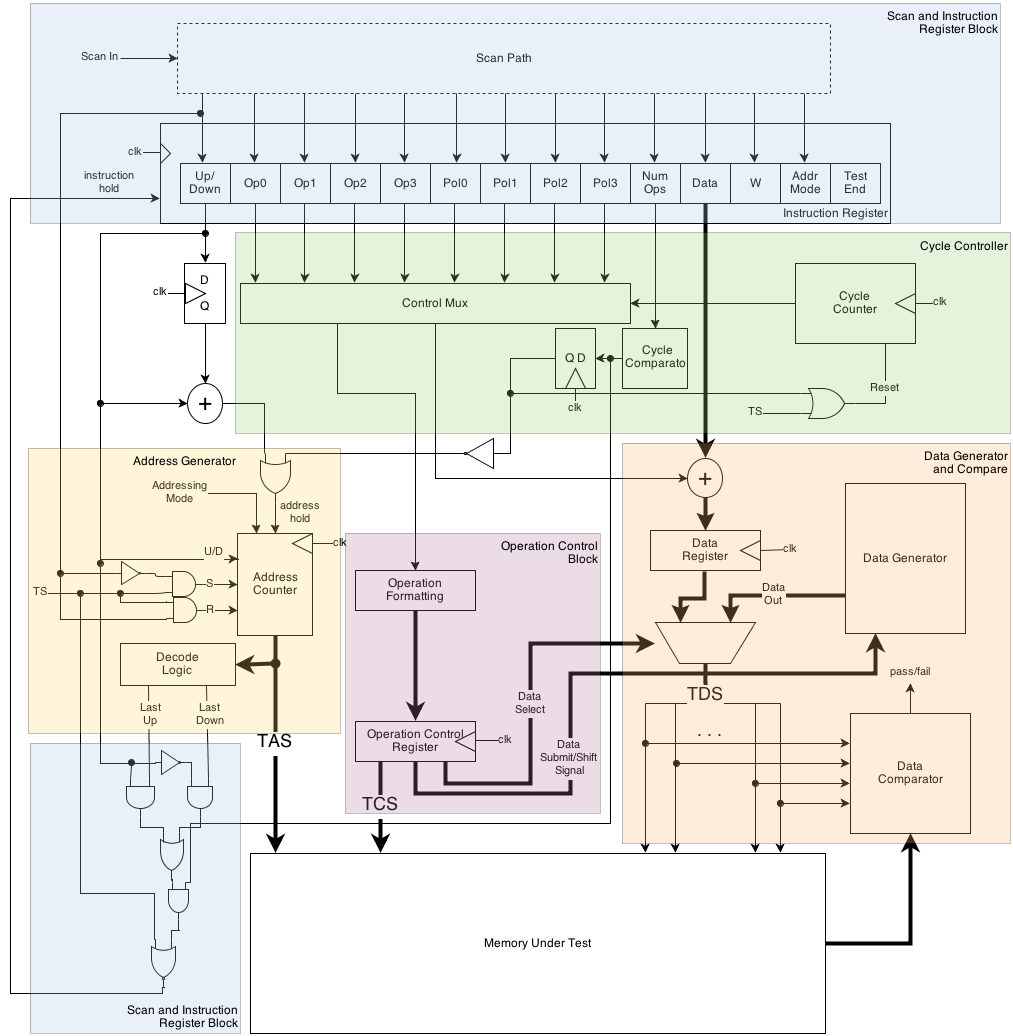
\includegraphics[scale=0.4]{pmbistall}
  \caption{Major Blocks of the PMBIST Design}
  \label{fig:pmbistall}
\end{figure}

\subsection{Scan and Instruction Register}
\label{sect:bg-blocks-scan-and-instruction-register}
Scan and the instruction register are the input mechanisms to the PMBIST.  In this design, the scan path is part of the chip-wide scan-chain that allows a tester to move data into BIST block.  The instruction register uses the data from the scan-chain to initiate a memory test.

\subsubsection{Instruction Register}
The instruction register contains all the fields required to initiate a memory test.  The four operation fields specify the March operation(s) to perform in the current March sequence while the number of operations (NO) field specifies how many March operations are in the current sequence.  The data field allows an 8-bit pattern to be written by the scan mechanism for a particular test, and the data polarity fields specify whether or not the data should be inverted for a particular March operation.  The address mode and up/down fields together determine the memory address counting method and direction.  Table \ref{tab:instreg} shows the fields and their corresponding bit positions within the register.

\begin{table}[H]
  \caption{Instruction Register Bit Fields}
  \centering
  \begin{tabular}{|p{1in}|c|p{3in}|}
  \hline
  %heading
  Name & Bit Position & Description \\
  \hline\hline
  Test End & [00:00] & Indicates end of test when all operations and addresses have been tested. \\ \hline
  Address Mode & [04:01] & Address counting method for address generator. \\ \hline
  Wait & [05:05] & Adds a wait state into the March test sequence. \\ \hline
  Data Field & [13:06] & 8-bit data for the March test. \\ \hline
  Number of Operations & [14:14] & Specifies the number of March operations in the current March test. \\ \hline
  Polarity 3 & [15:15] & Polarity of data for March operation 3. \\ \hline
  Polarity 2 & [16:16] & Polarity of data for March operation 2. \\ \hline
  Polarity 1 & [17:17] & Polarity of data for March operation 1. \\ \hline
  Polarity 0 & [18:18] & Polarity of data for March operation 0. \\ \hline
  Operation 3 & [22:19] & March operation for cycle 3. \\ \hline
  Operation 2 & [26:23] & March operation for cycle 2. \\ \hline
  Operation 1 & [30:27] & March operation for cycle 1. \\ \hline
  Operation 0 & [34:31] & March operation for cycle 0. \\ \hline
  Up/Down & [35:35] & Specifies the address counting direction. \\ \hline
  \end{tabular}
  \label{tab:instreg}
\end{table}

\subsubsection{Scan Path} 
The scan path is a test mechanism to serially transfer data from an external source into the PMBIST instruction register.  A separate scan clock will move data through a scan-chain until it aligns with the instruction register fields.  The test start (TS) signal will latch the scan data into the instruction register and begin the MBIST sequence.

\subsection{Cycle Controller}
\label{sect:bg-blocks-cycle-controller}
The cycle controller determines which March operation of those programmed in the IR should execute on the current memory address.  When all March operations have completed execution, the cycle controller generates a signal that allows the AC to move to the next test address.  The cycle controller then resets the March operation pointer to the first operation for the next address.   

\subsubsection{Control Mux}
The control mux receives all the operation and data polarity signals from the IR.  Using the CC's output as the mux control signal, the control mux selects the operation and polarity signal corresponding to the current cycle and outputs them to the operation formatting block and control register.  

\subsubsection{Cycle Counter}
The cycle counter increments a count which selects the March operation to execute.  The output of the cycle counter corresponds to the active March operation.  The cycle counter is incremented by the clock signal and can be reset by a TS signal or when the current March sequence has completed for the current memory address. 

\subsubsection{Cycle Comparison}
The cycle comparison unit compares the current cycle to the NO field of the instruction register.  When the cycle counter matches the NO field, the comparison block generates an active high signal that is stored in the cycle controller's local flip-flop.  The signal is also sent to the instruction register hold logic block.  



\subsection{Address Generator Block}
\label{sect:bg-blocks-address-generator}
The memory address to test and memory control signals are generated by the address and operation block.  The address decode block is used to generate the instruction register hold signal.  The hold signal maintains the instruction register's data until the current March sequence has completed for all memory address.  

\subsubsection{Address Counter}
The address counter indicates the memory address to test.  The direction of the address order can be programmed to increment or decrement through memory.  The CM is also programmable: linear up/down, pseudo-random sequence using LFSR, address complement, Gray coding, and 2\textsuperscript{i} CMs.  The address counter is used as an input to the circuits that generate the address complement, Gray coding  and 2\textsuperscript{\textit{i}} CM.  The address generator is described in more detail in Section \ref{sect:bg-modifications}.
 
\subsubsection{Address Decode Logic}
The address decode logic block determines if the address generated by the address counter is the last up (LU) or last down (LD) memory address for the current March sequence.  The decode logic uses the signals from the address programmer block to determine whether the sequence direction is up or down.   



\subsection{Data Generator and Compare}
\label{sect:bg-blocks-data-generator-and-compare-block}
Data can come from the instruction register or the data generator.  A mux select signal is generated based on the current operation.  For user data patterns, the data from the instruction register is selected and written to memory.  For NPSF patterns, the data generator outputs the word to be written to memory.  The comparator checks if the data read from memory matches what is expected and generates the pass/fail signal.

\subsubsection{Data Generator}
The data generator (DG) replaces the auxiliary memory in the proposed design.  Rather than use the scan-path to write the data background pattern to the MUT, the DG will dynamically create the pattern to allow the BIST to write the background to memory.  A more detailed description of the DG can be found in Section \ref{sec:dg}.

\subsubsection{Data Comparator}
Each read march element is checked with the data comparator.  The comparator accepts as inputs the TDS bus and the output of the MUT.  If the MUT output matches the TDS value, a pass signal is generated.  If there is any discrepancy, the fail signal is generated.  

\subsubsection{Polarity and Data Register}
The polarity signal from the current march operation is used to invert the data.  If the polarity signal is false (0), the data is unmodified and stored to the data register.  If the polarity signal is true (1), the data is inverted, then stored in the data register.  



\subsection{Operation Control Block}
\label{sect:bg-blocks-operation-control-block}
In some designs, the memory algorithm operation signals from the instruction register do not necessarily need to match the memory's control signals.  The operation formatting block can be used to translate the instruction register's operation code to the memory controller's signals such as write/read, enable and reset.

\subsubsection{Operation Formatting}
The operation formatting block converts the memory algorithm operation signal to explicit memory control signals such as read/write, enable and reset.  The output of this block passes to the control register.

\subsubsection{Operation Control Register}
The control register interprets the operation formatted instruction and sends any internal control signal to other blocks of the PMBIST.  In particular, this block sends the data mux select signal and controls the sequencing of the data generator.  It also writes the memory control signals to the TCS bus.  



\subsection{External Connections}
\label{sect:bg-blocks-external-connections}
Integration with the MUT and scan-path requires a few external connections.  The scan-path writes data to the instruction register for the test.  The MUT receives address, data and control signals from the memory BIST.

\subsubsection{Scan-Path Connection}
The scan-path receives data serially for the memory BIST.  The scan-path signals correspond to the instruction register fields.  When the scan-in data has been clocked into place, the instruction register will latch the data and begin its test.  

\subsubsection{Memory Under Test Connections}
The MUT connects to the MBIST through the test buses.  The connections provides the data, control signals and address to the memory and are connected to the memory input pins.  

\paragraph{Test Address Signals}
The test address signals (TAS) contain the memory address currently of interest to the test.  They can point to the read address for a comparison or the write address to store new data.

\paragraph{Test Control Signals}
The test control signals (TCS) are generated from the operator register.  The signals are formatted to work with the MUT.  The IR operation is translated to memory control signals such as read/write, reset and enable.  

\paragraph{Test Data Signals}
The test data signals (TDS) contain the data of interest to the test.  These signals are connected to the MUT's data input pins and the data comparator's input pins.  They are driven from the data register.  If an auxiliary memory is used, the data pins are driven from the outputs of the auxiliary memory.



